\documentclass[12pt]{article}
% in reality the next definitions lead to Heinrich's slatex and 
%from there to OMDOC declaration of the CD
\usepackage{multibib}
\usepackage{graphicx}
\newcommand{\mass}{\cal Mass}
\newcommand{\force}{\cal force}
\newcommand{\acceleration}{\cal acceleration}
\newcommand{\Massdensity}{\cal massdensity}
\newcommand{\Electricfield}{\cal electricfield}
\newcommand{\Temperature}{\cal temperature}
\newcommand{\Length}{\cal length}
\newcommand{\Time}{\cal time}
\newcommand{\ab}{\vspace{3mm}\\}
\newcites{own}{A. References to relevant work of the authors}
\newcites{others}{B. References to relevant external work}
\newcites{services}{C. Online Services}
\begin{document}
\centerline{\Large Physics Markup Language PhysML: the Concept} 
Editors for the respective chapters in brackets.
\\

Authors: Joseph B. Collins, Eberhard R. Hilf, and all those, participating in the
discussion, please add your name once you made more than three additions.
\tableofcontents
\newpage 
\section{Introduction}
(E.R.Hilf)

\section{Physics Description, General Part}
(E.R.Hilf)
\subsection{Definitions}
%\citeown{Hi-Ko-Sta}
\subsubsection{Physical Observable}
http://www.isn-oldenburg.de/\~hilf/lehre/index.html
for First term students
\textit{Introduction to Theoretical Physics, Measuring in Physics Theory
} 1998; Carl von Ossietzky University Oldenburg
\\


\subsubsection{Physics Objects}
\subsubsection{Physics Experiment}
\subsubsection{Physics Laws}
\section{A physical \textit{Type} for MML}
(Joe Collins) 
\subsection{Dimension Algebra}
\subsection{Clifford Algebra for physical objects}
General Part
%\cite{kleihaus}
\subsection{Application to vector-algebra}
\begin{figure}
  \begin{center} % vertical centering
    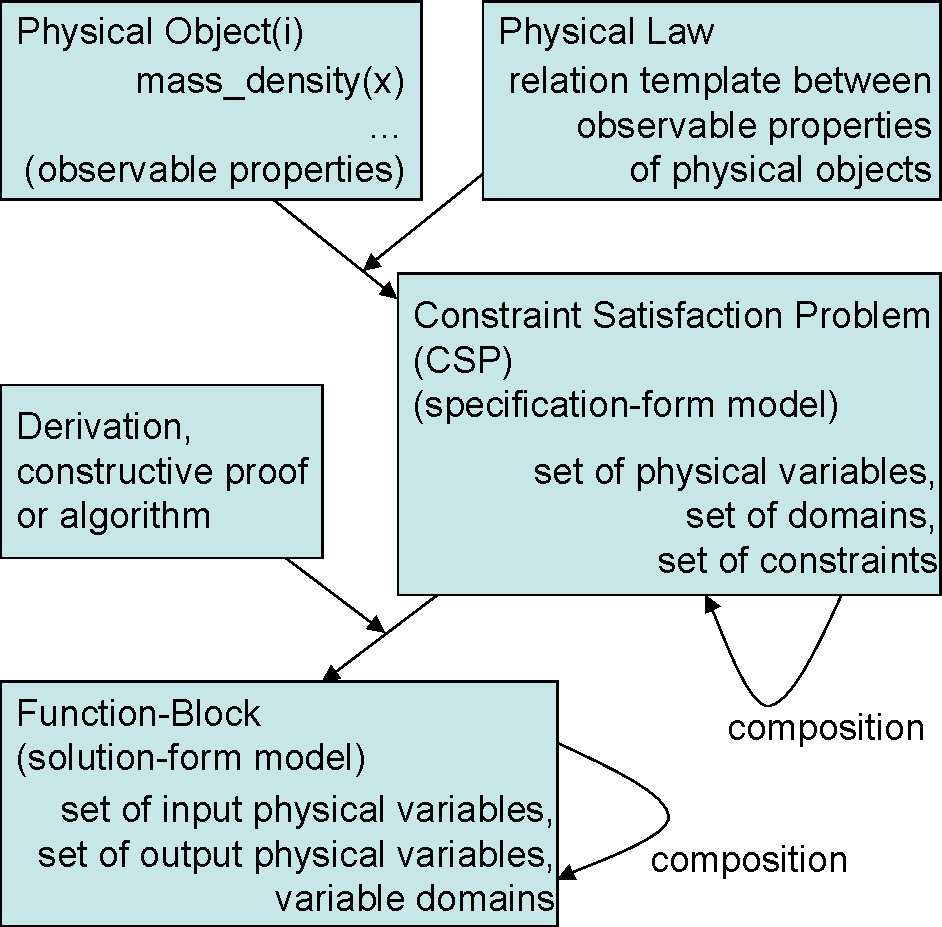
\includegraphics[clip=true, viewport=0 0 452 445, scale=0.9]{./MathModelOfMathModeling.pdf}
  \end{center}
\end{figure}
Example
\subsection{Differential forms}
(E.R.Hilf)
%\cite{hilf-2000-n}.

\section{Encoding Physics }
(M. Kohlhase)
\subsection{STeX encoding}
(H. Stamerjohanns)
\citeown{stex}
\subsection{OmDoc}
\section{Appendices}
\subsection{Appendix I: Observable Dictionary Prototype}
(E.R.Hilf)
\subsection{Appendix II: Physics law knowledge data base (Prototype}
(E.R. Hilf and J. Collins)
\subsection{Appendix 1: Example of Classical Physics: gravitation
  between two particles}

Object
Spherically_Symmetric Rigid Massive PhysicalObject:
name: A
mass_density: $\rho({\bf r}, t)$
mass: $\int \rho({\bf r}) d^3{\bf r}$
rigidity constraint: ${{d \rho({\bf r}, t)}\over{dt}} = 0$
spherical symmetry constraint: $\rho({\bf r}) = \rho(\left|{\bf r}\right|)$
ball constraint:  $\rho({\bf r}) = 0, \left|{\bf r}\right|>r_A$

?PhysML requires a binding construct local to described objects?


\subsection{The knowledge base: first step}
\section{Appendix III: Physics Objects knowledge data base (Prototype}
\section{Example}
\section{References}
\begin{small}
%\renewcommand\biblabelprefix{E}
% keine Kapitel fuer die einzelnen Abschnitte, sondern subsections:
\bibliographystyleown{alphadin}
\bibliographyown{physml-hilf,physml-joe,physml-kohlhase,physml-stamerjohanns}
%\renewcommand\biblabelprefix{}
\bibliographystyleothers{alphadin}
\bibliographyothers{physml-others}
\bibliographystyleservices{unsrtdin}
\bibliographyservices{physml-links}
\end{small}

\end{document}
